\chapter{Evaluation}\label{ch:evaluation}

\section{Evaluation Methodology}\label{sec:methodology}

For instance you can explain the hardware and software you used for your evaluation.
Explain all the details necessary for the readers to be able to reproduce your experiments.
Tables can be effective so use them accordingly.

\begin{table}[ht]
  \centering
  \caption{A table with lots of numbers.}{
  \rowcolors{3}{gray90}{}
  \resizebox{0.95\textwidth}{!}{
    {\renewcommand{\arraystretch}{1.3}
    \begin{tabular}{c>{\hspace{1pc}}c c c>{\hspace{1pc}}c c c} % https://tex.stackexchange.com/a/31704
      \toprule
      \multirow{2}{*}{Techniques we compare} & \multicolumn{3}{c}{Results (absolute values)} & \multicolumn{3}{c}{Results (relative to baseline)} \\
             & Area($mm^2$) & Delay($ns$) & Power($m W$) & Area(\%)  & Delay(\%) & Power(\%) \\
      \midrule
            Baseline &   347,329.19 &       1.62 &       15.84 &       --- &      --- &      --- \\
Proposed technique 1 &   412,263.87 &       1.65 &       16.17 &     18.69 &     1.85 &     2.12 \\
Proposed technique 2 &   370,972.35 &       2.42 &       17.95 &      6.80 &    49.38 &    11.00 \\
Proposed technique 3 &   356,694.82 &       1.98 &       16.00 &      2.69 &    22.22 &     1.06 \\
      \bottomrule
    \end{tabular}}\label{tab:example}
  }
}
\end{table}

\cref{tab:example} shows a lot of numbers.
Tables look better without vertical lines (some of you might have seen the linter message: ``Vertical rules in tables are ugly.'').
Also the odd rows are shaded in gray.
It greatly enhances the readability (especially with tables with many rows/columns) so is recommended to use it.

\section{Evaluation Results}\label{sec:results}

Quantitatively evaluate your proposed system/technique and discuss them.
Graphs are effective so use them accordingly.

\begin{figure}[ht]
  \centering
  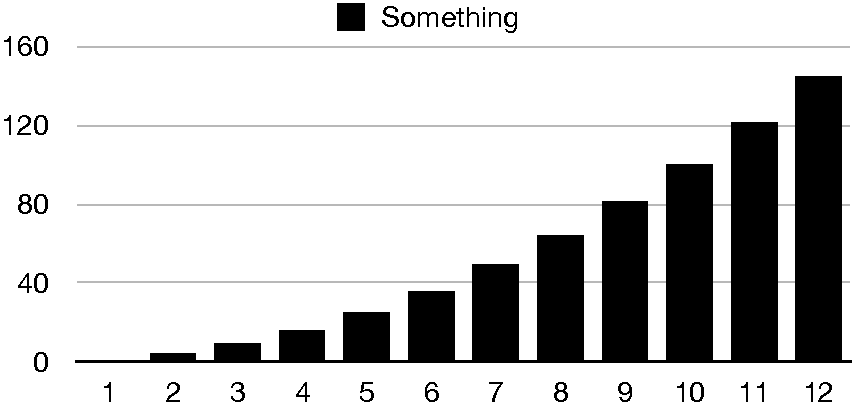
\includegraphics[width=0.9\textwidth]{examples/graphs/something}
  \caption{Trend of something.}\label{fig:something}
\end{figure}

If you look at \cref{fig:something}, we can see that the value of something is exponentially growing.
We present the detailed data of the evaluation results in \cref{ch:appendix2}.